\documentclass[11pt,a4paper]{article}
\usepackage[margin=1.8cm]{geometry}
\usepackage{tikz,graphicx,booktabs,amsmath,enumitem,hyperref,xcolor,pgfplots,caption,subcaption}
\pgfplotsset{compat=1.18}
\usetikzlibrary{shapes.geometric,arrows.meta,positioning,fit}
\captionsetup{font=small,labelfont=bf}
\setlist{nosep,leftmargin=*}
\setlength{\parskip}{2pt}\setlength{\parindent}{0pt}
\definecolor{ink}{HTML}{1F2933}\definecolor{muted}{HTML}{7B8794}\definecolor{accent}{HTML}{2563EB}\definecolor{grid}{HTML}{E4E7EB}
\pgfplotsset{every axis/.append style={axis line style={muted},tick style={muted},major grid style={grid},
  tick label style={font=\scriptsize,text=ink},label style={font=\scriptsize,text=ink},ymajorgrids,xmajorgrids=false,major x grid style={draw=none},axis lines=left,enlarge x limits=false}}
\title{\vspace{-1.4cm}Catan Bot}
\author{Team Blanc}
\date{17 October 2026}
\begin{document}\maketitle\vspace{-0.9cm}

\begin{abstract}\noindent
Our agent scores every legal move by its exact expected value over dice, development-card draws and robber steals,
then searches its own turn to depth 3. Positions are scored by a hand-written evaluation plus eight times the
log-odds of a small learned win-probability model. Setup placements are chosen by playing out the remaining setup
for both players. The hand-written evaluation alone won 77.7\% against F. The learned correction raised this to 81\%,
and the setup rollouts to 85.7\% against F and 70.1\% against O on the leaderboard. The final agent won 83.5\% of 600
games against F in the official harness with no games over the time limit.
\end{abstract}

\section{Introduction}
Two findings shaped the design. First, catanatron's alpha-beta bots search F's evaluation function and still win
only 37\% to 50\% against F, even with no time limit. F ranks positions well but its score is not a win probability,
so deeper search over it compounds its errors. Second, a learned win-probability model inside a short search
reached 75\% against F and then stopped improving, although its test loss continued to fall (Section~\ref{sec:neg}).
A hand-written evaluation with tuned weights outperformed it, and the sum of the two outperformed both.

\section{Agent}
\begin{figure}[t]\centering
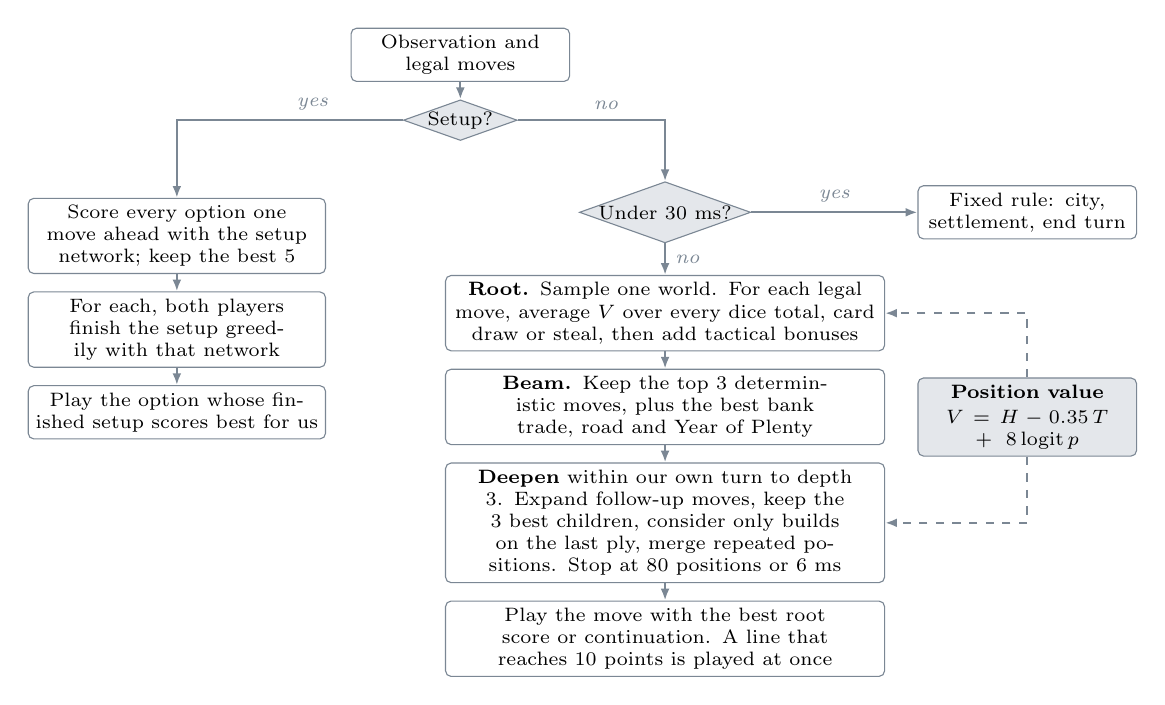
\begin{tikzpicture}[font=\scriptsize, node distance=2.2mm,
  base/.style={draw=muted,rounded corners=2pt,align=center,inner sep=2.5pt,fill=white},
  wide/.style={base,text width=5.4cm}, side/.style={base,text width=3.6cm}, small/.style={base,text width=2.6cm},
  dec/.style={draw=muted,diamond,aspect=2.8,align=center,inner sep=0pt,fill=grid},
  arr/.style={-{Latex[length=1.5mm]},muted,thick}, lab/.style={font=\scriptsize\itshape,text=muted}]
\node[small] (in) at (-2.6,0) {Observation and legal moves};
\node[dec, below=of in] (setup) {Setup?};
\node[side] (s1) at (-6.2,-2.3) {Score every option one move ahead with the setup network; keep the best 5};
\node[side, below=of s1] (s2) {For each, both players finish the setup greedily with that network};
\node[side, below=of s2] (s3) {Play the option whose finished setup scores best for us};
\node[dec] (time) at (0,-2.0) {Under 30 ms?};
\node[small] (rule) at (4.6,-2.0) {Fixed rule: city, settlement, end turn};
\node[wide, below=4mm of time] (m1) {\textbf{Root.} Sample one world. For each legal move, average $V$ over every dice total, card draw or steal, then add tactical bonuses};
\node[wide, below=of m1] (m2) {\textbf{Beam.} Keep the top 3 deterministic moves, plus the best bank trade, road and Year of Plenty};
\node[wide, below=of m2] (m3) {\textbf{Deepen} within our own turn to depth 3. Expand follow-up moves, keep the 3 best children, consider only builds on the last ply, merge repeated positions. Stop at 80 positions or 6 ms};
\node[wide, below=of m3] (m4) {Play the move with the best root score or continuation. A line that reaches 10 points is played at once};
\node[small, fill=grid] (V) at (4.6,-4.6) {\textbf{Position value}\\[1pt] $V = H - 0.35\,T$\\ $+\;8\,\mathrm{logit}\,p$};
\draw[arr] (in)--(setup);
\draw[arr] (setup.west) -| node[lab,pos=0.2,above]{yes} (s1.north);
\draw[arr] (setup.east) -| node[lab,pos=0.3,above]{no} (time.north);
\draw[arr] (s1)--(s2); \draw[arr] (s2)--(s3);
\draw[arr] (time)--node[lab,above]{yes}(rule);
\draw[arr] (time)--node[lab,right]{no}(m1);
\draw[arr] (m1)--(m2); \draw[arr] (m2)--(m3); \draw[arr] (m3)--(m4);
\draw[arr,dashed] (V.north) |- (m1.east);
\draw[arr,dashed] (V.south) |- (m3.east);
\end{tikzpicture}
\caption{How the agent chooses a move. Setup decisions use rollouts with the setup network. Main-game decisions
score every move by its exact expectation over chance and then search deeper within our own turn, using the position
value $V$ at every node.}\label{fig:flow}
\end{figure}
\paragraph{Move scoring under chance.} The agent samples one world consistent with its observation. For each legal
move it enumerates every random outcome with its probability: the 11 dice totals, each development card the unseen
pile can yield, and each card a robber can steal. It scores each resulting position and takes the expectation.
Further sampled worlds would not change any score, because the evaluation reads only public information and the
card-draw expectation already covers every unseen card.

\paragraph{Same-turn search.} The opponent cannot act during our turn, so a sequence of trades and builds is a
single-player problem. The agent expands the 3 highest-scoring deterministic continuations, plus the best bank
trade, road and Year of Plenty, whose value appears only once the build they enable is visible. It deepens
iteratively to depth 3 and stops at 80 positions or 6\,ms. The final ply considers builds only. A transposition table
merges identical positions reached by different orders. A move's score is the best continuation found, and any
line that reaches 10 victory points is played immediately.

\paragraph{Position evaluation.} A position $s$ is scored as
\[ V(s) = H(s) - 0.35\,T(s) + 8\cdot\mathrm{logit}\,p(s). \]
$H$ is the hand-written evaluation in Table~\ref{tab:terms}, in units of roughly one twelfth of a victory point.
$T$ measures how close the opponent is to affording its next point-scoring build at its port rates, scaled up as
it approaches 10 points. $p$ is the logit average of two networks with 76 inputs and hidden layers of 64 and 32,
trained with cross-entropy on game outcomes from 8.3M positions and from 400k further self-play games. Their inputs
include per-resource production with the robber applied, ports, hand, points, army and road state, settlement spots
reachable now and after one road, and development cards.

\begin{table}[h]\centering\small
\resizebox{\linewidth}{!}{\begin{tabular}{llr}\toprule
Term & Definition & Weight \\\midrule
Points & $12\,\mathrm{VP}_{\text{ours}} - 10\,\mathrm{VP}_{\text{opp}}$, our count includes our hidden VP cards & fixed \\
Production & $\phi\cdot w_p\,(P + 0.08\sum_r \min(1, p_r/0.08) - 0.8\,P_{\text{opp}} - 0.064\,D_{\text{opp}})$ & $w_p = 18$ \\
Expansion & $\phi\cdot w_e\,(7 b_0 + 3 b_1 + 0.25\min(3,n_0) + 0.08\min(3,n_1))$ & $w_e = 0.714$ \\
Hand readiness & $w_h\,\max_g v_g\,(0.8\,e^{-0.65 d_g} + 0.2\,e^{-0.65\max(0,d_g-t_g)}) + 0.12\,w_h N - 0.1\max(0,N-7)$ & $w_h = 0.9$ \\
Largest Army & $w_a \min(k, k^*-1)$ while not held, plus a value per unplayed knight & $w_a = 2.50$ \\
Development cards & $1.3$ Road Building, $1.5$ Year of Plenty, $1.8$ Monopoly & fixed \\
Longest Road & $0.25\min(4, \text{road length})$ while not held & fixed \\\bottomrule
\end{tabular}}
\caption{Terms of $H$. $P$ is expected cards per roll and $p_r$ its share for resource $r$; $D$ counts distinct
resources. $b_0, b_1$ are the best spot production reachable now and after one road, $n_0, n_1$ their counts.
For each build goal $g$ with value $v_g$, $d_g$ is the number of missing cards and $t_g$ the number obtainable by
port trades. $N$ is hand size, $k$ played knights and $k^*$ the current army threshold.
$\phi = \max(0.3,\,1-0.12\max(0,\mathrm{VP}-4))$ moves weight from income to points late in the game.}
\label{tab:terms}
\end{table}

The four weights $w$ and three tactical coefficients were tuned by hill climbing, 400 games per round, maximising
the lower of the win rates against F and a tactical heuristic opponent. They were frozen before held-out testing.

\paragraph{Setup placement.} For each settlement and road decision in the setup, the agent scores every option one
move ahead with a third network, which we call the setup network, keeps the best 5, completes the setup greedily for both players
with the same network, and plays the option whose completed setup scores highest. The choice therefore accounts for
the opponent's next placement.

\paragraph{Time management.} Each decision has a hard deadline of $\min(60, t-15)$\,ms, where $t$ is the time left.
A partly scored move list returns the best completed score. Below 30\,ms the agent plays a fixed rule: city, then
settlement, then end turn.

\section{Experiments}\label{sec:exp}
All win rates are against F through the official evaluation harness with both seats per board, unless stated.
At 2,000 games the 95\% interval is about $\pm1.9$ points, at 1,000 games $\pm2.5$, and at 400 games $\pm4.4$.

\paragraph{Value of each decision type.} We replaced one decision type of an early agent at a time with F's choice
or a random choice, over 2,000 games each. The agent won 65.0\%. With F's robber it won 69.9\%, with F's main turn
49.1\%, with a random setup 10.4\% and with a random robber 36.2\%. All of the agent's advantage came from main-turn
play, its own robber was worse than F's, and the setup was worth about 55 points. This set our priorities.

\paragraph{The evaluation function.} Figure~\ref{fig:ladder} shows win rate as each part of the evaluation is added.
The hand-written score with a one-move lookahead won 71.8\%, already close to the learned model inside the full
search at 75.0\%. Adding the opponent-threat term $T$, the knight, robber and Monopoly bonuses and an army-focused weight preset
raised it to 76.1\%, and the same-turn search with tuned weights to 77.7\%. On the same 1,000 boards, the learned
correction raised the search from 79.0\% to 81.0\%. With setup rollouts the agent reached 85.7\% on the leaderboard.

\begin{figure}[h]\centering
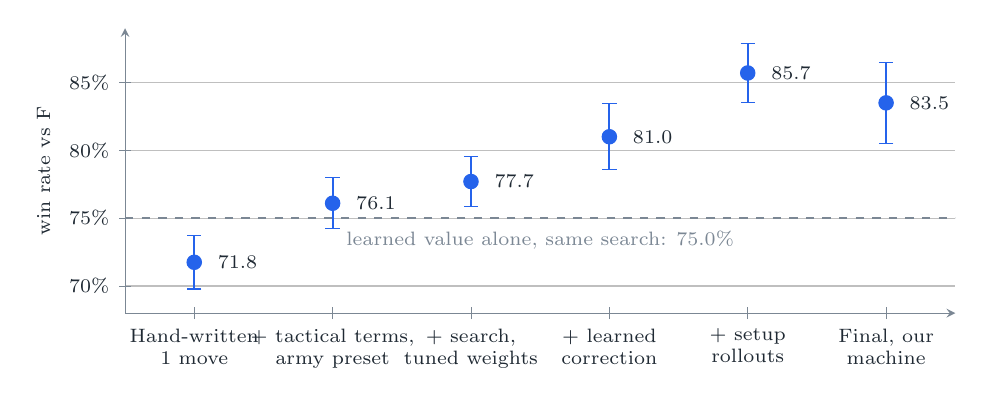
\begin{tikzpicture}
\begin{axis}[width=\linewidth,height=5.2cm,ymin=0.68,ymax=0.89,ytick={0.70,0.75,0.80,0.85},
  yticklabel={\pgfmathparse{\tick*100}\pgfmathprintnumber[fixed,precision=0]{\pgfmathresult}\%},
  xtick={1,2,3,4,5,6},xmin=0.5,xmax=6.5,ylabel={win rate vs F},
  xticklabels={{Hand-written\\1 move},{+ tactical terms,\\army preset},{+ search,\\tuned weights},{+ learned\\correction},{+ setup\\rollouts},{Final, our\\machine}},
  xticklabel style={align=center,font=\scriptsize}]
\addplot[muted,dashed,thick,domain=0.5:6.5,samples=2]{0.750};
\node[font=\scriptsize,text=muted,anchor=north] at (axis cs:3.5,0.748) {learned value alone, same search: 75.0\%};
\addplot[color=accent,only marks,mark=*,mark size=2.6pt,error bars/.cd,y dir=both,y explicit,error bar style={color=accent,thick}]
 coordinates {(1,0.7175)+-(0,0.0197) (2,0.761)+-(0,0.0187) (3,0.777)+-(0,0.0182) (4,0.810)+-(0,0.0243) (5,0.857)+-(0,0.0217) (6,0.835)+-(0,0.0297)};
\node[font=\scriptsize,text=ink,anchor=west] at (axis cs:1.1,0.7175) {71.8};
\node[font=\scriptsize,text=ink,anchor=west] at (axis cs:2.1,0.761) {76.1};
\node[font=\scriptsize,text=ink,anchor=west] at (axis cs:3.1,0.777) {77.7};
\node[font=\scriptsize,text=ink,anchor=west] at (axis cs:4.1,0.810) {81.0};
\node[font=\scriptsize,text=ink,anchor=west] at (axis cs:5.1,0.857) {85.7};
\node[font=\scriptsize,text=ink,anchor=west] at (axis cs:6.1,0.835) {83.5};
\end{axis}\end{tikzpicture}
\caption{Win rate against F as parts of the evaluation are added, with 95\% intervals. Points 1 to 3 are 2,000
held-out games each, point 4 is 1,000 local games, point 5 the leaderboard's 1,000, and point 6 600 games on a
machine with the evaluation processor. Point 6 also adds setup-road rollouts and a memory fix. Seeds differ between
points, so adjacent steps below about 3 points are not individually significant.}\label{fig:ladder}
\end{figure}

We tested the hand-written weights by halving or raising each of the production, hand and army weights by half,
over 400 games each. Win rate against F stayed within 1.3 points of the base value of 72.3\%, inside the 400-game
interval. The evaluation is therefore insensitive to its
exact weights, which suggests its value lies in the terms it contains rather than in tuning. A later test that raised
the production weight by half in the final agent won 47.5\% head to head against the unchanged agent over 200 games,
consistent with this. The weight on the learned correction does matter. Without it the agent won 76.5\%, with
weights 2 and 8 it won 82.2\% and 82.3\%, and with 16 it fell to 79.7\%. At 16 the network outweighs the
hand-written terms and the search inherits its ranking errors.


\paragraph{Final changes.} In the last round each candidate played 200 games against the previous submission,
200 against a sibling agent and 200 against F. Extending the setup rollout to both roads won 57.0\% against the
previous submission and was kept. Rollout for the first road only won 55.0\%, two opponent-model variants of the
setup won 49.0\% and 52.0\%, and raising the production weight by half won 47.5\%. Over 600
games on a machine with the evaluation processor it won 80.8\% with 17 games over the time limit. Section~\ref{sec:inf}
describes the cause. With the fix the same policy won 83.5\% with none.


\section{Negative results}\label{sec:neg}
\paragraph{Learned evaluation alone.} The network alone, one move ahead, won 39\%. Inside the same-turn search it won
62\%, and retraining on its own games raised this to 75\%. Larger networks, 2.5 times more games, wider and deeper
search and 47 extra features all landed between 72\% and 77\% while test loss fell from 0.4193 to 0.4081. Inside the
search, the median value gap between the best and second-best move was 0.008, but four equally accurate networks
differed by 0.016 on the same position and agreed on the move only 60\% to 72\% of the time. The search needs the
model to rank sibling positions, which test loss does not measure.

\paragraph{Raw state as input.} A network on the raw 639-number game state reached a lower test loss than the feature
network, 0.434 against 0.439, and won 9.9\% against it. The search selected positions outside its training
distribution, where its values were unreliable.

\paragraph{Reinforcement learning.} Networks trained by self-play reached 72\% against F one move ahead and 52\%
against the supervised network inside the same search, a tie within the interval. Training toward the network's own
one-move estimates instead of game outcomes reduced strength in proportion to how much weight the estimates got.
Networks on the raw state memorised boards, with training loss 0.09 and validation loss 0.88.

\paragraph{A C simulator.} We reimplemented the rules in C for data generation. It matches catanatron on every move
over 100,000 games and runs about 200 times faster per move. It removed data generation as a bottleneck, but more
data did not move the learned model past its plateau.

\section{Inference and the time budget}\label{sec:inf}
An agent that runs out of time plays random moves for the rest of the game, so we treated CPU time as part of
strength. An earlier leaderboard submission ran out of time in 21 of 1,000 games at 382\,ms per game on average,
well below the allowance, which told us the problem was spikes rather than average cost.

\paragraph{Search budget.} The search spends 4\% of the time left above a 100\,ms reserve, with a cap of 6\,ms and 80
positions per decision. Every decision also has a hard deadline of $\min(60, t-15)$\,ms. If the deadline arrives
while moves are still being scored, the agent returns the best move scored so far, and below 30\,ms it plays the fixed
rule without copying the game. Discards are never searched. In an earlier agent, discards are made one card at a time
and keep the turn with us, so the search deepened through each one, costing about 26\,ms per discard and 39\% of that
agent's CPU time.

\paragraph{Feature cache.} The feature code cached each board's tile and production data, keyed by the board object's
identity. The official harness gives the agent a new copy of the game at every decision, so the cache gained one
entry per decision and never shrank. Python's garbage-collection pauses grew with it, from 32\,ms after 200 decisions
to 365\,ms after 3,000. Our own test runner reused one board object and never showed the fault. Capping the cache at 8
boards leaves every feature value unchanged, which we checked over 100 freshly copied boards. Over 600 games against F
on a machine with the evaluation processor, it reduced games over the time limit from 17 to 0 and mean CPU from 392 to
371\,ms per game.

\paragraph{Threads and loading.} Every thread the agent starts counts against its clock, so the agent pins the numeric
libraries to one thread before numpy loads. Loading is not charged to any game, but anything initialised lazily is
charged to the first decision that uses it. In one candidate, running its opening model once during loading cut its first
call from 16.8\,ms to 3.4\,ms.

\paragraph{Evaluation cost.} Each position evaluation is one call to the hand-written score and one small network.
A searched decision makes about 23 of them. We tried the setup network's larger feature set at the leaves as well. It
won 52.4\% head to head over 2,000 games but cost 1.6 to 2 times the CPU, 205 against 157\,ms per game, so the leaves
keep the smaller network.

\paragraph{Public material.} catanatron by Bryan Collazo, GPL-3.0, in the organisers' patched build; numpy;
scikit-learn. Iterative deepening, quiescence and transposition tables follow standard chess-engine practice as in
Stockfish; no code was copied. Language models wrote much of our code.

\end{document}
